% !TeX root = RJwrapper.tex
\title{List-columns in \texttt{data.table}: Nesting and unnesting data tables
and vectors}
\author{by Tyson S. Barrett}

\maketitle

\abstract{%
The use of list-columns in data frames and tibbles is well documented,
providing a cognitively efficient way to organize results of complex
data (e.g.~statistical models, data summaries, even graphics) with
corresponding data. This allows the data to be of variable sizes without
overly complicating or adding redundancies to the structure of the data.
In turn, this can improve the reliability to appropriately analyze the
data. Because of its efficiency and speed, being able to use
\texttt{data.table} to work with list-columns would be beneficial in
many data contexts (e.g.~to reduce memory usage in large data sets).
Herein, list-columns are shown to be created in a data table using the
\texttt{by} argument in \texttt{data.table} and \texttt{purrr::map()}.
The behavior of the \texttt{data.table} approach is compared to the
\texttt{dplyr::group\_nest()} function. Results using
\texttt{bench::mark()} show the speed and efficiency of using
\texttt{data.table} to work with list-columns.
}

% Any extra LaTeX you need in the preamble

\hypertarget{introduction}{%
\section{Introduction}\label{introduction}}

The use of \emph{list-columns} in data frames and tibbles provides a
cognitively efficient way to organize complex data (e.g.~several
statistical models, groupings of text, data summaries, or even graphics)
with corresponding data in a concise manner. It has become a common
approach to wrangling data in the \texttt{tidyverse}, with functions
across \texttt{dplyr} and \texttt{tidyr} providing functionality to work
with list-columns \citep{R-dplyr,R-tidyr,jenny}. This format is often
called ``nested'' data, where information is, in essence, nested within
a column of data.

For example, list-columns can be used to nest data regarding students
within classrooms, players within teams, measures within individuals,
and text within chapters. This allows the user to do certain data
manipulations within each group in a consistent, controlled manner. This
can ensure that accidentally including data from other groups does not
occur. Furthermore, nesting can reduce the difficulty to appropriately
analyze the data stored in the list-column. Using functions like
\texttt{lapply()} or \texttt{purrr::map*()} makes further analysis of
the nested data more intuitive and error-free.

Because of its efficiency and speed, being able to use
\texttt{data.table} to work with list-columns would be beneficial in
many data contexts (e.g.~to reduce memory usage in large data sets,
increase speed of calculations). Herein, I demonstrate how one can
create list-columns in a data table using the \texttt{by} argument in
\texttt{data.table} (using a custom function) and the
\texttt{purrr::map*()} functions. I further highlight the
\texttt{dplyr::group\_nest()} function and show a slightly more
efficient approach when using a data table. Using
\texttt{bench::mark()}, I assess the speed and efficiency of using
\texttt{data.table} to work with list-columns.

This article relies on several powerful R packages, including
\texttt{data.table}, \texttt{dplyr}, \texttt{bench}, \texttt{tidyr},
\texttt{rticles}, \texttt{stringr}, \texttt{ggplot2},
\texttt{ggbeeswarm}, \texttt{ggrepel}, \texttt{performance},
\texttt{rvest}, and \texttt{lobstr}
\citep{R-data.table,R-dplyr,R-bench,R-tidyr,R-rticles,R-stringr,R-ggbeeswarm,R-ggrepel,R-ggplot2,R-rvest,R-performance,R-lobstr}.

\hypertarget{example-data}{%
\section{Example Data}\label{example-data}}

Throughout much of this paper, I demonstrate the use of
\emph{list-columns} in \texttt{data.table} using data from
\href{nbastuffer.com}{NBA Stuffer}. These data are downloaded, providing
information on players from the 2017-2018 and 2018-2019 seasons. To do
so, I first read in the HTML data, then extract the tables with player
data by year (using a short custom function), add indicators, and then
combine each into a single data table. Each step is shown in the code
below.

\begin{Schunk}
\begin{Sinput}
url_2018 <- "https://www.nbastuffer.com/2017-2018-nba-player-stats/"
url_2019 <- "https://www.nbastuffer.com/2018-2019-nba-player-stats/"
players_2018 <- read_html(url_2018)
players_2019 <- read_html(url_2019)

extract_fun <- function(html){
  tabs <- html_nodes(html, "table")[2] %>% 
    html_table(fill = TRUE)
  tabs[[1]] 
}

player_2018 <- 
  extract_fun(players_2018) %>% 
  mutate(year = 2018,
         AGE = as.numeric(AGE))
player_2019 <- 
  extract_fun(players_2019) %>% 
  mutate(year = 2019)

players <- 
  bind_rows(player_2018, player_2019) %>% 
  clean_names() %>% 
  rename(ppg = ppg_points_points_per_game,
         apg = apg_assists_assists_per_game) %>% 
  data.table()
\end{Sinput}
\end{Schunk}

\noindent Below is a subset of this imported data set, showing only four
of the variables and the first six rows.

\begin{Schunk}
\begin{Soutput}
#>         full_name team year  mpg  ppg apg
#> 1:   Aaron Brooks  Min 2018  5.9  2.3 0.6
#> 2:   Aaron Gordon  Orl 2018 32.9 17.6 2.3
#> 3: Aaron Harrison  Dal 2018 25.9  6.7 1.2
#> 4:  Aaron Jackson  Hou 2018 34.5  8.0 1.0
#> 5:    Abdel Nader  Bos 2018 10.9  3.0 0.5
#> 6:  Adreian Payne  Orl 2018  8.5  4.2 0.0
\end{Soutput}
\end{Schunk}

\hypertarget{nesting-with-data.table}{%
\section{\texorpdfstring{Nesting with
\texttt{data.table}}{Nesting with data.table}}\label{nesting-with-data.table}}

In \texttt{dplyr}, the \texttt{group\_nest()} function is valuable when
creating list-columns based on a grouping variable. It takes the data by
group and puts it all in a list-column. Figure \ref{process} highlights
the process of taking a data frame and creating a nested data frame with
a list-column. That is, all data from variables \texttt{x}, \texttt{y},
and \texttt{z} relating to each group is split into a distinct data
frame and stored within the \texttt{data} column.

\begin{figure}[b]
  \centering
  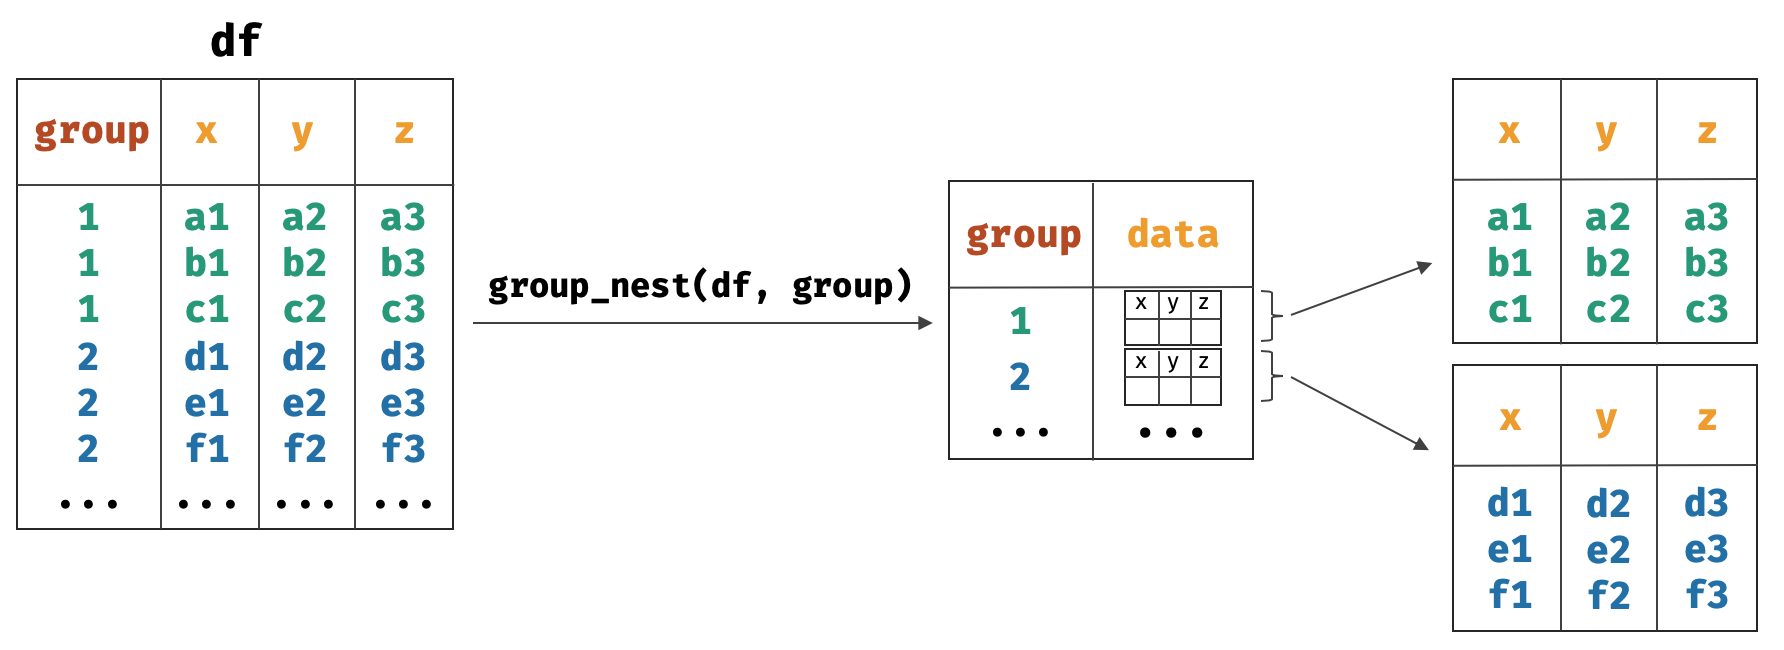
\includegraphics[width=\textwidth]{fig_process.png}
  \caption{Diagram of one approach to creating a list-column in a data frame (i.e. creating a nested data frame).}
  \label{process}
\end{figure}

Overall, this function is efficient and fast but---by relying on
\texttt{data.table}---it can be somewhat faster. This will be shown
using the following function, which relies solely on the syntax of
\texttt{data.table}, using the \texttt{j} and \texttt{by} arguments as
shown below.

\begin{Schunk}
\begin{Sinput}
group_nest_dt <- function(dt, ..., .key = "data"){
  stopifnot(is.data.table(dt))

  by <- substitute(list(...))
  
  dt <- dt[, list(list(.SD)), by = eval(by)]
  setnames(dt, old = "V1", new = .key)
  dt
}
\end{Sinput}
\end{Schunk}

First thing to note, is that in the data table, we create a list within
a list containing the \texttt{.SD} special object. This object is all
the data in the data table except for the variables that are in the
\texttt{by} argument. The \texttt{by} argument, before being evaluated
within the data table, first becomes an unevaluated list of bare
variable names and then evaluate it within the \texttt{data.table}
syntax. In essence, this function takes a data table, then creates a
list of the data table per group specified in the \texttt{by} argument.

\begin{Schunk}
\begin{Sinput}
head(group_nest_dt(players, team))
\end{Sinput}
\begin{Soutput}
#>    team         data
#> 1:  Min <data.table>
#> 2:  Orl <data.table>
#> 3:  Dal <data.table>
#> 4:  Hou <data.table>
#> 5:  Bos <data.table>
#> 6:  Ind <data.table>
\end{Soutput}
\end{Schunk}

The syntax and output are nearly identical to the
\texttt{dplyr::group\_nest()} function but has data tables in the
list-column instead of tibbles.

\begin{Schunk}
\begin{Sinput}
head(group_nest(players, team))
\end{Sinput}
\begin{Soutput}
#> # A tibble: 6 x 2
#>   team  data              
#>   <chr> <list>            
#> 1 Atl   <tibble [44 x 30]>
#> 2 Bos   <tibble [37 x 30]>
#> 3 Bro   <tibble [41 x 30]>
#> 4 Cha   <tibble [34 x 30]>
#> 5 Chi   <tibble [43 x 30]>
#> 6 Cle   <tibble [49 x 30]>
\end{Soutput}
\end{Schunk}

Given both perform very similar data manipulations, it is of interest to
see if there are differences in memory and speed performance. Figure
\ref{speed} presents the timings from \texttt{bench::mark()} across the
two approaches, showing \texttt{group\_nest\_dt()} is often faster,
although differences for this size of data set are not meaningful. The
memory allocated is also very similar, with \texttt{group\_nest\_dt()}
allocating \ensuremath{4.61704\times 10^{5}} and \texttt{group\_nest()}
allocating \ensuremath{3.42832\times 10^{5}}.

\begin{figure}[tb]
  \centering
  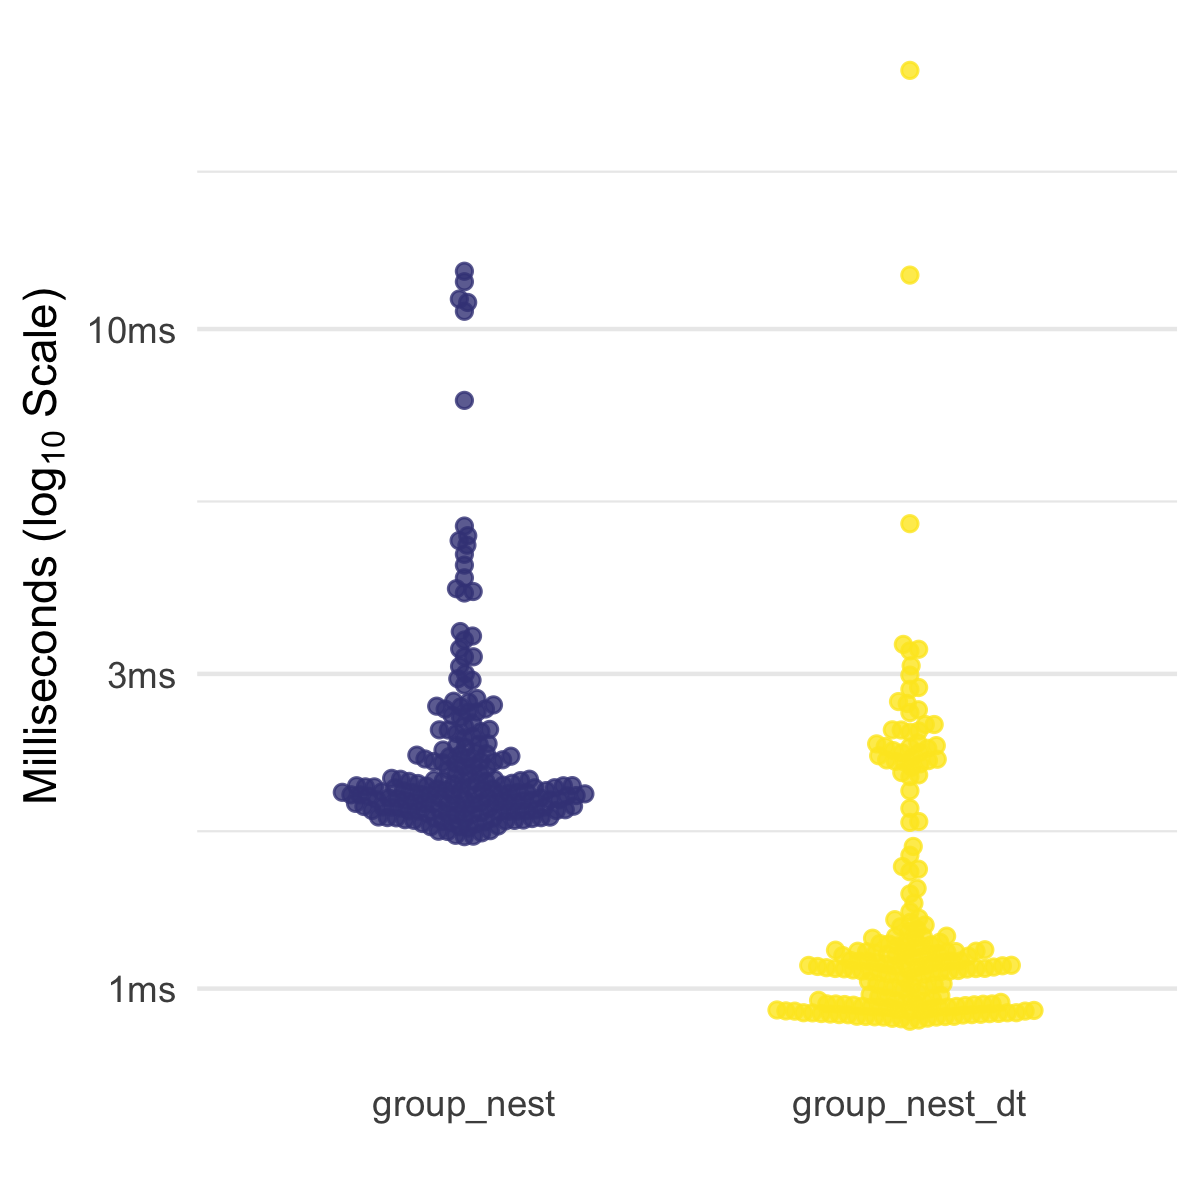
\includegraphics[width=0.6\textwidth]{timings_manuscript.png}
  \caption{Speed comparisons for each nesting approach. Note the scale of the y-axis is log$_{10}$.}
  \label{speed}
\end{figure}

This nesting approach can be used with multiple grouping variables too.
For example, I show how a user could nest by both \texttt{team} and
\texttt{year}, as is done below.

\begin{Schunk}
\begin{Sinput}
head(group_nest_dt(players, team, year))
\end{Sinput}
\begin{Soutput}
#>    team year         data
#> 1:  Min 2018 <data.table>
#> 2:  Orl 2018 <data.table>
#> 3:  Dal 2018 <data.table>
#> 4:  Hou 2018 <data.table>
#> 5:  Bos 2018 <data.table>
#> 6:  Ind 2018 <data.table>
\end{Soutput}
\end{Schunk}

\hypertarget{analyses-within-the-nested-data}{%
\subsection{Analyses within the Nested
Data}\label{analyses-within-the-nested-data}}

Often, the nested data can provide an intuitive format to run several
analyses to understand key features of the data within the groups.
Below, the relationship between points-per-game and assists-per-game for
each team and year is modeled and then the \(R^2\) of the models are
extracted. Since \texttt{performance::r2()} provides two versions of
\(R^2\), I then grab only the first of the two types.

\begin{Schunk}
\begin{Sinput}
players_nested <- group_nest_dt(players, team, year)
players_nested[, ppg_apg    := purrr::map(data, ~lm(ppg ~ apg, data = .x))]
players_nested[, r2_list    := purrr::map(ppg_apg, ~performance::r2(.x))]
players_nested[, r2_ppg_apg := purrr::map_dbl(r2_list, ~.x[[1]])]
head(players_nested)
\end{Sinput}
\begin{Soutput}
#>    team year         data ppg_apg      r2_list r2_ppg_apg
#> 1:  Min 2018 <data.table>    <lm> <r2_generic>  0.4662060
#> 2:  Orl 2018 <data.table>    <lm> <r2_generic>  0.4357684
#> 3:  Dal 2018 <data.table>    <lm> <r2_generic>  0.4305347
#> 4:  Hou 2018 <data.table>    <lm> <r2_generic>  0.6967150
#> 5:  Bos 2018 <data.table>    <lm> <r2_generic>  0.6043402
#> 6:  Ind 2018 <data.table>    <lm> <r2_generic>  0.6060465
\end{Soutput}
\end{Schunk}

\noindent This produces two list-columns (\texttt{ppg\_apg} and
\texttt{r2\_list}) and a numeric vector (\texttt{r2\_ppg\_apg}) all
organized by team and year. This information is then readily available
to plot. For example, one can look at how related points-per-game and
assists-per-game are by team and year---in essence, showing which teams
have players who both score and assist. The example plot is shown in
Figure \ref{exfig}.

\begin{Schunk}
\begin{Sinput}
players_nested %>% 
  dcast(team ~ year, value.var = "r2_ppg_apg") %>% 
  ggplot(aes(`2018`, `2019`, group = team)) +
    geom_point() +
    geom_text_repel(aes(label = team)) +
    geom_abline(slope = 1) +
    coord_fixed(ylim = c(0,1),
                xlim = c(0,1))
\end{Sinput}
\end{Schunk}

\begin{figure}[tb]
  \centering
  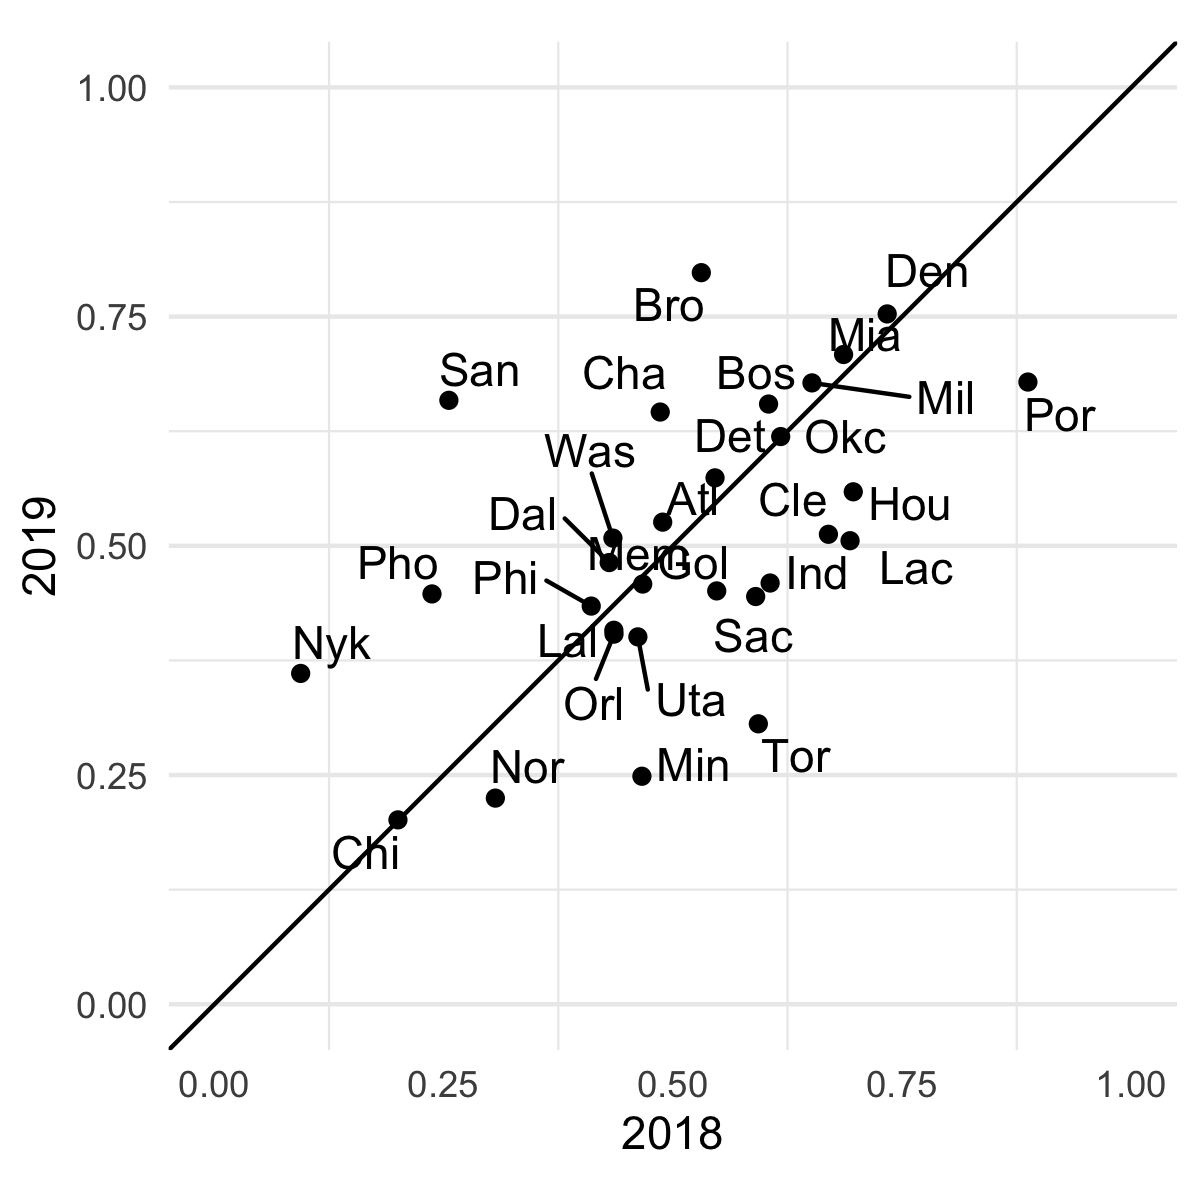
\includegraphics[width=0.5\textwidth]{ex_fig.png}
  \caption{Example analysis performed using nested data to provide information for each team and year.}
  \label{exfig}
\end{figure}

\hypertarget{unnesting-with-data.table}{%
\section{\texorpdfstring{Unnesting with
\texttt{data.table}}{Unnesting with data.table}}\label{unnesting-with-data.table}}

After performing the manipulations or analyses within the nest, it can
often be necessary to unnest to finalize analyses. Again, like with
\texttt{group\_nest\_dt()}, the \texttt{unnest\_dt()} function below
relies solely on the syntax of \texttt{data.table}, using the \texttt{j}
and \texttt{by} arguments as shown below.

\begin{Schunk}
\begin{Sinput}
unnest_dt <- function(dt, col, id){
  stopifnot(is.data.table(dt))
  
  by <- substitute(id)
  col <- substitute(unlist(col, recursive = FALSE))
  
  dt[, eval(col), by = eval(by)]
}
\end{Sinput}
\end{Schunk}

This function can be used to unnest a data table, like the
\texttt{players\_nested} data table from earlier, where the nested
column can be a data table, data frame, or tibble. Below, the
\texttt{data} column in the table is unnested by \texttt{team} and
\texttt{year} and then a few of the variables are selected for
demonstration purposes.

\begin{Schunk}
\begin{Sinput}
players_unnested <- unnest_dt(players_nested, 
          col = data, 
          id = list(team, year))
players_unnested[, .(team, year, full_name, pos, age, gp, mpg)]
\end{Sinput}
\begin{Soutput}
#>       team year          full_name pos   age gp  mpg
#>    1:  Min 2018       Aaron Brooks  PG 33.00 32  5.9
#>    2:  Min 2018     Andrew Wiggins  SF 22.00 82 36.3
#>    3:  Min 2018      Anthony Brown  SF 25.00  1  3.7
#>    4:  Min 2018       Cole Aldrich   C 29.00 21  2.3
#>    5:  Min 2018       Derrick Rose  PG 29.00  9 12.4
#>   ---                                               
#> 1223:  Det 2019     Svi Mykhailiuk   G 21.84  3  6.6
#> 1224:  Det 2019      Zaza Pachulia   C 35.16 68 12.9
#> 1225:  Det 2019 Glenn Robinson III G-F 25.26 47 13.0
#> 1226:  Det 2019          Ish Smith   G 30.77 56 22.3
#> 1227:  Det 2019       Khyri Thomas   G 22.92 26  7.5
\end{Soutput}
\end{Schunk}

\begin{figure}[tb]
  \centering
  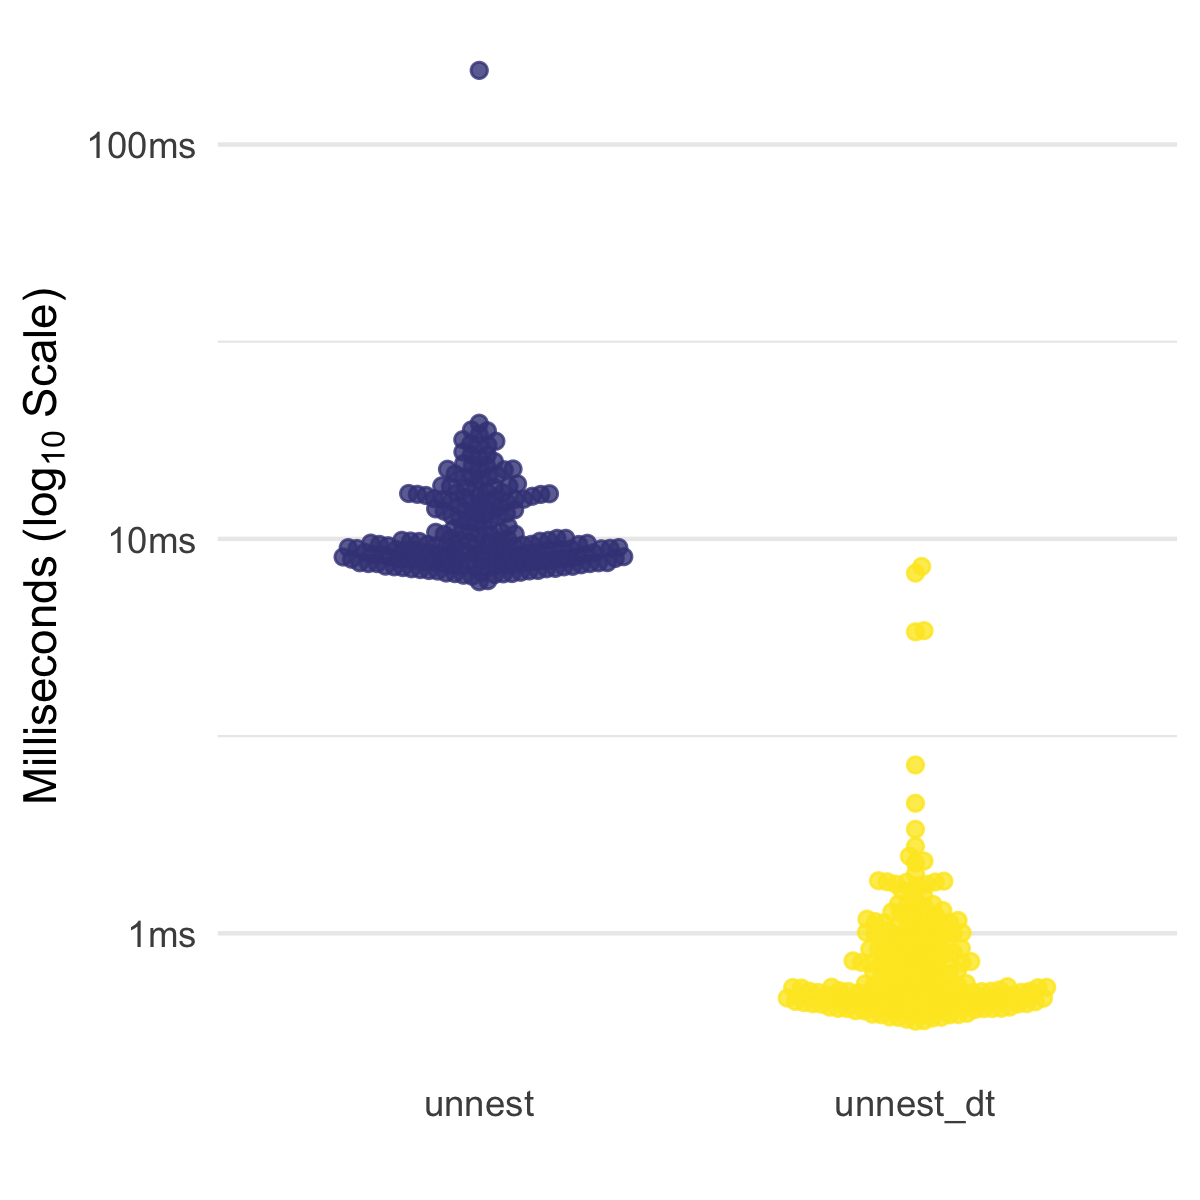
\includegraphics[width=0.6\textwidth]{timings_unnest_manuscript.png}
  \caption{Speed comparisons for each unnesting approach. Note the scale of the y-axis is log$_{10}$.}
  \label{speed2}
\end{figure}

Again, this function is quick and efficient. Figure \ref{speed2}
presents the timings from \texttt{bench::mark()} across the two
unnesting approaches, showing the \texttt{data.table} approach is much
faster. The memory allocated is about half for the \texttt{data.table}
approach here, with \texttt{unnest\_dt()} allocating
\ensuremath{9.33648\times 10^{5}} and \texttt{tidyr::unnest()}
allocating \ensuremath{1.914208\times 10^{6}}.

\hypertarget{unnesting-vectors-with-data.table}{%
\subsection{\texorpdfstring{Unnesting Vectors with
\texttt{data.table}}{Unnesting Vectors with data.table}}\label{unnesting-vectors-with-data.table}}

A slight variation of this function can be used for list-columns with
atomic vectors instead of data tables. A function like the following
works well.

\begin{Schunk}
\begin{Sinput}
unnest_vec_dt <- function(dt, cols, id, name){
  stopifnot(is.data.table(dt))
  
  by <- substitute(id)
  cols <- substitute(unlist(cols, 
                            recursive = FALSE))
  
  dt <- dt[, eval(cols), by = eval(by)]
  setnames(dt, old = paste0("V", 1:length(name)), new = name)
  dt
}
\end{Sinput}
\end{Schunk}

In \texttt{players\_nested}, the \texttt{r2\_list} column is a list of
numeric vectors. This can be unnested as shown below, providing the two
measures of \(R^2\) per team per year.

\begin{Schunk}
\begin{Sinput}
unnest_vec_dt(players_nested, 
              cols = list(r2_list), 
              id = list(team, year), 
              name = "r2")
\end{Sinput}
\begin{Soutput}
#>      team year        r2
#>   1:  Min 2018  0.466206
#>   2:  Min 2018 0.4280779
#>   3:  Orl 2018 0.4357684
#>   4:  Orl 2018 0.4025783
#>   5:  Dal 2018 0.4305347
#>  ---                    
#> 116:  Lac 2019 0.4808586
#> 117:  Phi 2019 0.4342685
#> 118:  Phi 2019 0.4106964
#> 119:  Det 2019 0.5740963
#> 120:  Det 2019  0.550435
\end{Soutput}
\end{Schunk}

\hypertarget{memory-usage-of-list-columns}{%
\section{Memory Usage of
List-Columns}\label{memory-usage-of-list-columns}}

Last item to demonstrate herein is the computer memory usage of
different formats of data tables with the same data. We can use the
following large data sets in wide format, nested wide format, long
format, and nested wide format to make brief comparisons.

\begin{Schunk}
\begin{Sinput}
# Wide
wide_format <- data.table(id = 1:1e6,
                          x1 = rnorm(1e6),
                          x2 = rnorm(1e6),
                          y1 = rnorm(1e6),
                          y2 = rnorm(1e6),
                          group = rbinom(1e6, 1, .5))
nested_wide_format <- group_nest_dt(wide_format, group)

# Long
long_format <- melt.data.table(wide_format, 
                               id.vars = c("id", "group"),
                               measure.vars = c("x1", "x2", "y1", "y2"))
nested_long_format <- group_nest_dt(long_format, group)
\end{Sinput}
\end{Schunk}

I use the \texttt{lobstr} package to assess the object size of each
format of the same data, shown in Table \ref{memtab}. Not surprising,
the memory usage of nested data is lower than for its none nested
corresponding data. This is directly related to the reduction in
redundancies in the data otherwise there. That is, the nested data has
far fewer rows containing the \texttt{group} variable. That, alone, in
this large data saves memory. For example, the size of a single column
of the \texttt{group} variable in wide format is 4 MB; and in long
format it is 16 MB By reducing a single variable in this case, we save
several megabytes of memory.

\begin{table}[ht]
\centering
\caption{Memory usage for each format of the same data} 
\label{memtab}
\begin{tabular}{lr}
  \toprule
Format & Memory (MB) \\ 
  \midrule
Wide Format & 40.0 \\ 
  Nested Wide Format & 36.0 \\ 
  Long Format & 80.0 \\ 
  Nested Long Format & 64.0 \\ 
   \bottomrule
\end{tabular}
\end{table}

\hypertarget{discussion}{%
\section{Discussion}\label{discussion}}

List-columns are a useful approach to structuring data into a format
that can be safely cleaned, manipulated, and analyzed by groups. It also
provides for a more cognitively efficient way for a user to understand
their data, allowing large data to be represented more concisely within
groups.

The \texttt{tidyverse} provides several functions to work with nested
data, which are relatively quick and efficient. For most data
situations, these functions will do all that a user will need. However,
in some situations, \texttt{data.table} can perform needed manipulations
and analyses that cannot otherwise be done or that would take too long
to complete. In these situations, and for users that prefer to use
\texttt{data.table}, this tutorial can help provide direction in using
list-columns.

Furthermore, as expected, the memory usage of nested data is lower than
for its none nested corresponding data. This is due to the reduction in
the redundancies present in wide and long format. This suggests that it
is not only the cognitive benefits to the user that makes this format
more efficient.

\hypertarget{limitations}{%
\subsection{Limitations}\label{limitations}}

There are some notable limitations to list-columns in general, and in
\texttt{data.table} specifically. First, the three custom functions
built on \texttt{data.table} presented herein are not well-tested and
are certainly not expected to work in each case where
\texttt{dplyr::group\_nest()}, \texttt{tidyr::unnest()}, and other tidy
functions would work. Rather, they were presented to show how a user can
leverage the speed and efficiency of \texttt{data.table} to create, and
work with, list-columns.

Second, it is important to realize that nested data can remove the
ability to use vectorization across groups. Depending on the analyses
being conducted, this may slow down the computation to the point that
nested data actually is a hindrance to performance.

Finally, when using list-columns in tibbles, the print method provides
the dimensions of each corresponding nested tibble. This method is
helpful in understanding the nested data without any need to extract it.
This could be a minor, but valuable, update to the print method in
\texttt{data.table}.

\hypertarget{conclusions}{%
\section{Conclusions}\label{conclusions}}

The use of list-columns in \texttt{data.table} is very similar to that
in the \texttt{tidyverse}. It provides speed and efficiency in both
nesting and unnesting the data, and can be used with the
\texttt{purrr::map*()} and other powerful functions.

\bibliography{barrett}


\address{%
Tyson S. Barrett\\
Utah State University\\
2800 Old Main Hill\\ Logan, UT 84322\\
}
\href{mailto:tyson.barrett@usu.edu}{\nolinkurl{tyson.barrett@usu.edu}}

